\documentclass[11pt,A4Paper]{article}
\usepackage[utf8]{inputenc}
\usepackage[a4paper,margin=1.5cm,top=2cm]{geometry}
\usepackage{graphicx}
\graphicspath{/Users/JohnnyLin/Desktop/Dzmitry_Lab /UROPS/uropsReport/figures}
\usepackage{float}
\usepackage{gensymb}
\usepackage{datetime}
\setlength{\parindent}{0pt}
\usepackage{appendix}
\usepackage{amsmath}
\usepackage[stable]{footmisc} %for footnote in title
\usepackage[hidelinks]{hyperref}
\usepackage{multirow,multicol}
\usepackage{adjustbox}
\usepackage{fancyhdr}
\pagestyle{fancy}
% \fancyhf{}
\rhead{UROPS-CQT}
\lhead{Lin Zhonglin A0222183N}

\title{UROPS Report}
\author{Lin Zhonglin \hspace{1cm} A0222183N}
\usdate{}

\begin{document}
\maketitle

\section{Introduction}


\section{Background}
\begin{enumerate}
    \item introduction of our lab -> refer to the trapped Ytterbium ion paper
    \item what did I do
    \item how do the stuff I did relate to the lab in general
\end{enumerate}

\section{Building and tuning 638nm Grating Stabilized Compact Laser}
\subsection{Theory}
\begin{enumerate}
    \item lasers in general
    \item diode laser + reference that compact laser paper
    \item Gaussian beam optics
    \item geometric optics -> different lens system 
\end{enumerate}

\subsubsection{Gaussian optics}
different modes of a laser + relate to mode hopping in "Tuning laser" section

..\subsection{Building and Tuning The Laser}
\cite{compactGratingDiodeLaser}theory about tuning a diode laser: frequency jumping + how I adjusted temp, current, angle of grating to tune frequency + discuss how the process can be automated.
temp: don't let temp go below due point (about 17) 

\begin{figure}[H]
    \centering
    \includegraphics[width=0.5\textwidth]{638laser.HEIC}
    \caption{638nm laser}
    \label{fig:638laser}
\end{figure}

\subsection{Fiber Coupling}
(Coupling laser into a single-mode optical fiber) 
brief theory + detailed steps of it being done + how can be done better (automation) 
2. Coupling a beam into a fibre 
    1. 用laser pen
    2. 在两个位置,分别用两个自由度调
    3. 最后提高功率,取出激光笔,四个扭左右转一转直到有光从fiber出来
    
1. Using a power meter 
    1. Adjust the 4 knobs independently → find the maximum point for each knob
    2. Walking the beam (horizontal and vertical → do separately)
        1. defining one mirror and trying to compensate with the other mirror 
            1. if cannot compensate, the detuned mirror is turned in the wrong direction
            2. Else try until maximum combination found

About local maxima: 

1. In the initial stage: scan through a larger range to find the global maxima among the many local maxima 
2. Later state: constantly check for whether the maxima being optimised is a local maximum → by turning left and right a bit more

# Cleaning Fibre

- Possible reasons for the fibre being dirty:
    - Dirt attached due to electrostatic attraction
- Draw out a new section of cloth
- Draw figure 8 multiple times until clean
- Look at the fibre using both side lighting and perpendicular lighting
- Spray acetone onto cloth and continue with figure 8 movement
    - Maybe debris on fibre is soluble

sources: 
1. https://www.researchgate.net/post/How-to-couple-laser-light-into-a-single-mode-fiber
2. https://www.youtube.com/watch?v=kQvhbJbDG0M


\subsection{Beam Characterisation}
\begin{enumerate}
    \item knife edge measurement (rational, procedure, put up some photos)
    \item photo diode (attach code in annex)
    \item can compare the two methods
    \item fitting measurement data with gaussian approx to recover gaussian beam parameters 
    \item possibility of automating the process
    \item beam shaping: anamorphic prisms / lens
\end{enumerate}

\subsubsection{Beam Collimation}
brief literature review + what I did + what it can be done better if higher precision is needed
\begin{enumerate}
    \item using a iris for horizontal and vertical alignment
    \item measure the umerical aperture of the fiber + tuning a fiber mount lens for collimation + finding the gaussian parameters again thorugh beam spot characterisation and back-fitting
\end{enumerate}




\subsection{Section conclusion}
what is this particular 638nm used in the lab for? -> for switching the trapped ion's state right? 


\section{Building and tuning Reference Cavity for 935nm laser}
\subsection{Theory}
theory about Fabry–Pérot cavity + relevant paper 




\subsection{Optical cavity allignment and coupling}
detailed steps + photos of apparatus + possble steps for better alignment

mode matching -> see notion for detail

\subsection{Sideband Checking}
discuss how can the cavity be used for this + detailed description of setup + pictures (if have time)



\subsection{Wavelength Measurement}
figure out how to use it to measure wavelength

\ssection{Frequency Locking a Laser}
discuss: laser frequency locking mechanisms + how can the cavity be used for this + detailed description of setup + pictures (if have time)

Stabilisation arrangements 

1. coupling to an external, high-Q cavity
    1. a fraction of the output beam is coupled into a high-Q Fabry-Perot resonator and redirected back into the diode laser
    2. geometry of this kind can provide radiation with a linewidth below 10kHz 
    3. relative high level of technical complexity 
2. coupling to a diffraction grating
    1. linewidth reduction to the 100kHz level
    2. the light diffracted from a grating is coupled back into the diodech

\\

Tunable lasers have multiple wavelength-selecting elements such as piezo-controlled etalons and gratings. Typically, the length of the lasing cavity is controlled by a voltage sent to a piezo-electric transducer. The laser-cavity length can change because of a number of factors such as temperature changes, and mechanical vibrations. These factors affect the laser-frequency stability. The standard method of frequency-locking involves a two step process outlined in \cite{PDH1983} and \cite{PDHintro}. 
\\
\\

\begin{figure}[H]
    \centering
    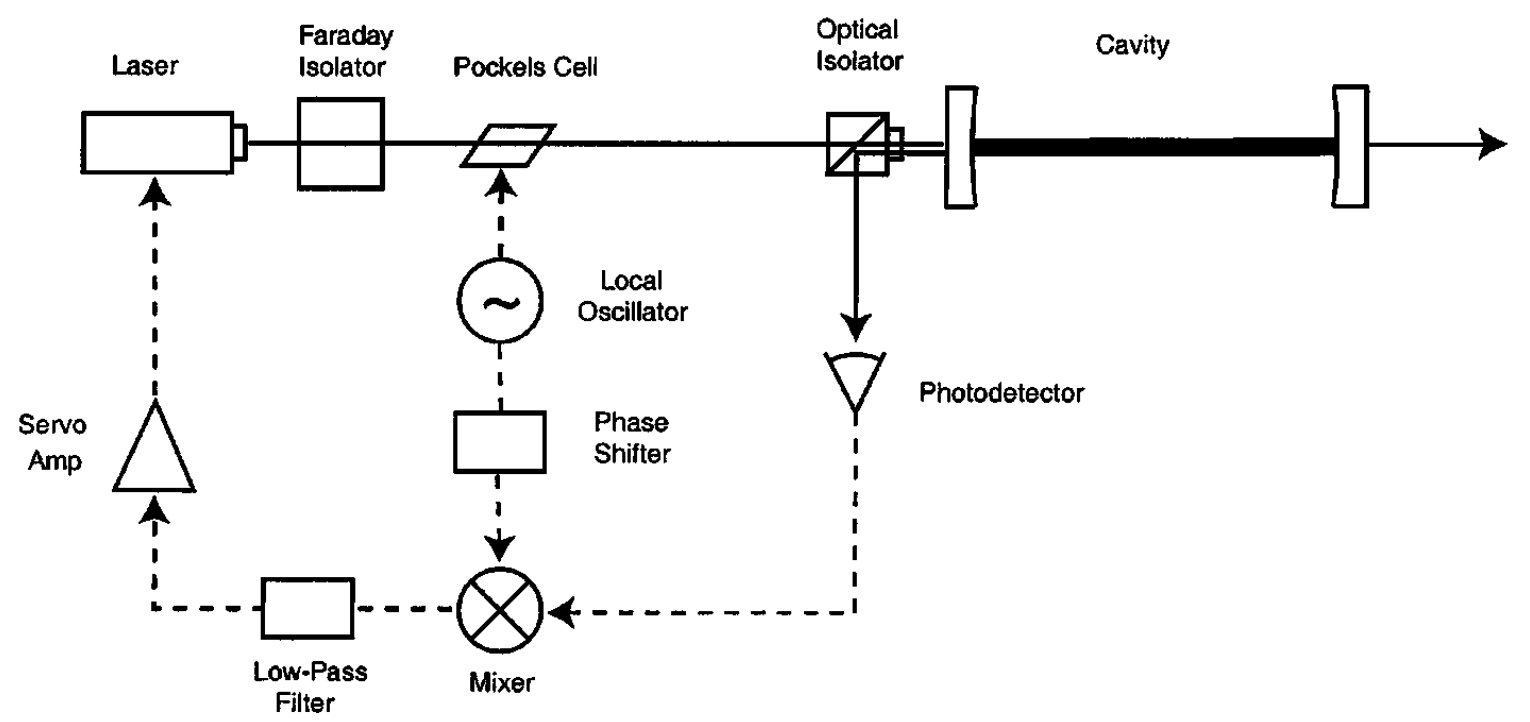
\includegraphics[width=\textwidth]{PDHlayout.png}
    \caption{The basic layout for locking a cavity to a laser. Solid lines are optical paths and dashed lines are signal paths. The signal going to the laser controls its frequency \cite{PDHintro}}
    \label{fig:PDHlayout}
\end{figure}
\subsection{EOM (Electro-optic Modulator)}
% put basic intro to an EOM here 
In certain types of crystals it is possible to effect a change in the index of refraction that is proportional to the applied electric field. This is the linear electro-opic effect (also known as the Pockels effect). Applying a modulated electric field across such a nonlinear crystal (usualy the KDP type) and passing a beam of laser through the crystal leads to the laser beam being modulated in phase. (detail see: \cite{fundamentalsOfPhotonics}

\subsubsection{Theory and Model}
When a time-varying electric field is applied to the nonlinear crystal inside the EOM, the index of refraction $n$ changes in a sinusoidal manner resulting in phase modulation of the laser beam passing through the crystal. Consider the following short mathematical example to see that phase modulation is equivalent to frequency: 
\\
% 见激光原理for this part
Suppose instantaneous electric field at a point of EM wave of a laser beam: 
\begin{align*}
    E_c(t) = A_c cos(\omega_c T + \varphi_c)
\end{align*}
With phase modulation (assume sinusoidal modulation), we have final phase of the electric field of the EM wave: 
\begin{align*}
    \psi(t) &= \omega_c t + \varphi_c + \Delta \varphi (t) \\
            &= \omega_c t + \varphi_c + m_{\varphi} sin(\omega_m t)
\end{align*}
So the modulated electric field now becomes: 
\begin{align}
    E(t) &= A_c cos[ \omega_c t + m_{\varphi} sin(\omega_m t) + \varphi_c] \label{eqn:7.1.9}\\
         &= A_c cos\left\{  \int_0^t [ \omega_c + \Delta ]\omega(t)] dt + \varphi_c \right\} \\
\end{align}
where, 
\begin{equation*}
    \Delta \omega (t) = \frac{d\Delta \varphi (t)}{dt}
\end{equation*}
If we do Fourier transform to Eqn \ref{eqn:7.1.9}, we obtain in frequency space: 
\begin{equation}
    E(\omega) = A_c J_0(m) \delta(\omega - \omega_c) + A_c\sum_{n=1}^\infty J_m(m) \left\{ \delta[\omega-(\omega_c + n\omega_m)] +(-1)^n\delta[\omega-(\omega_c-n\omega_m)]\right\}
    \label{eqn:7.1.10}
\end{equation}

Eqn \ref{eqn:7.1.10} shows that when a single-frequency laser beam is modulated by a sinusoidal frequency, the modulated beam in frequency space comprises of the unmodulated frequency $\omega_0$ and infinite sidebands. Sideband frequency spacing is $\omega_m$, modulation frequency. 
% actually not sure about this, need to double check the math
Sideband amplitudes are determined by the Bessel function $J_n(m)$. (See Fig \ref{fig:EOMsidebandTheory}) What's of concern in this case is that EOM phase modulation produces frequency sidebands of laser beam. 

\begin{figure}[H]
    \centering
    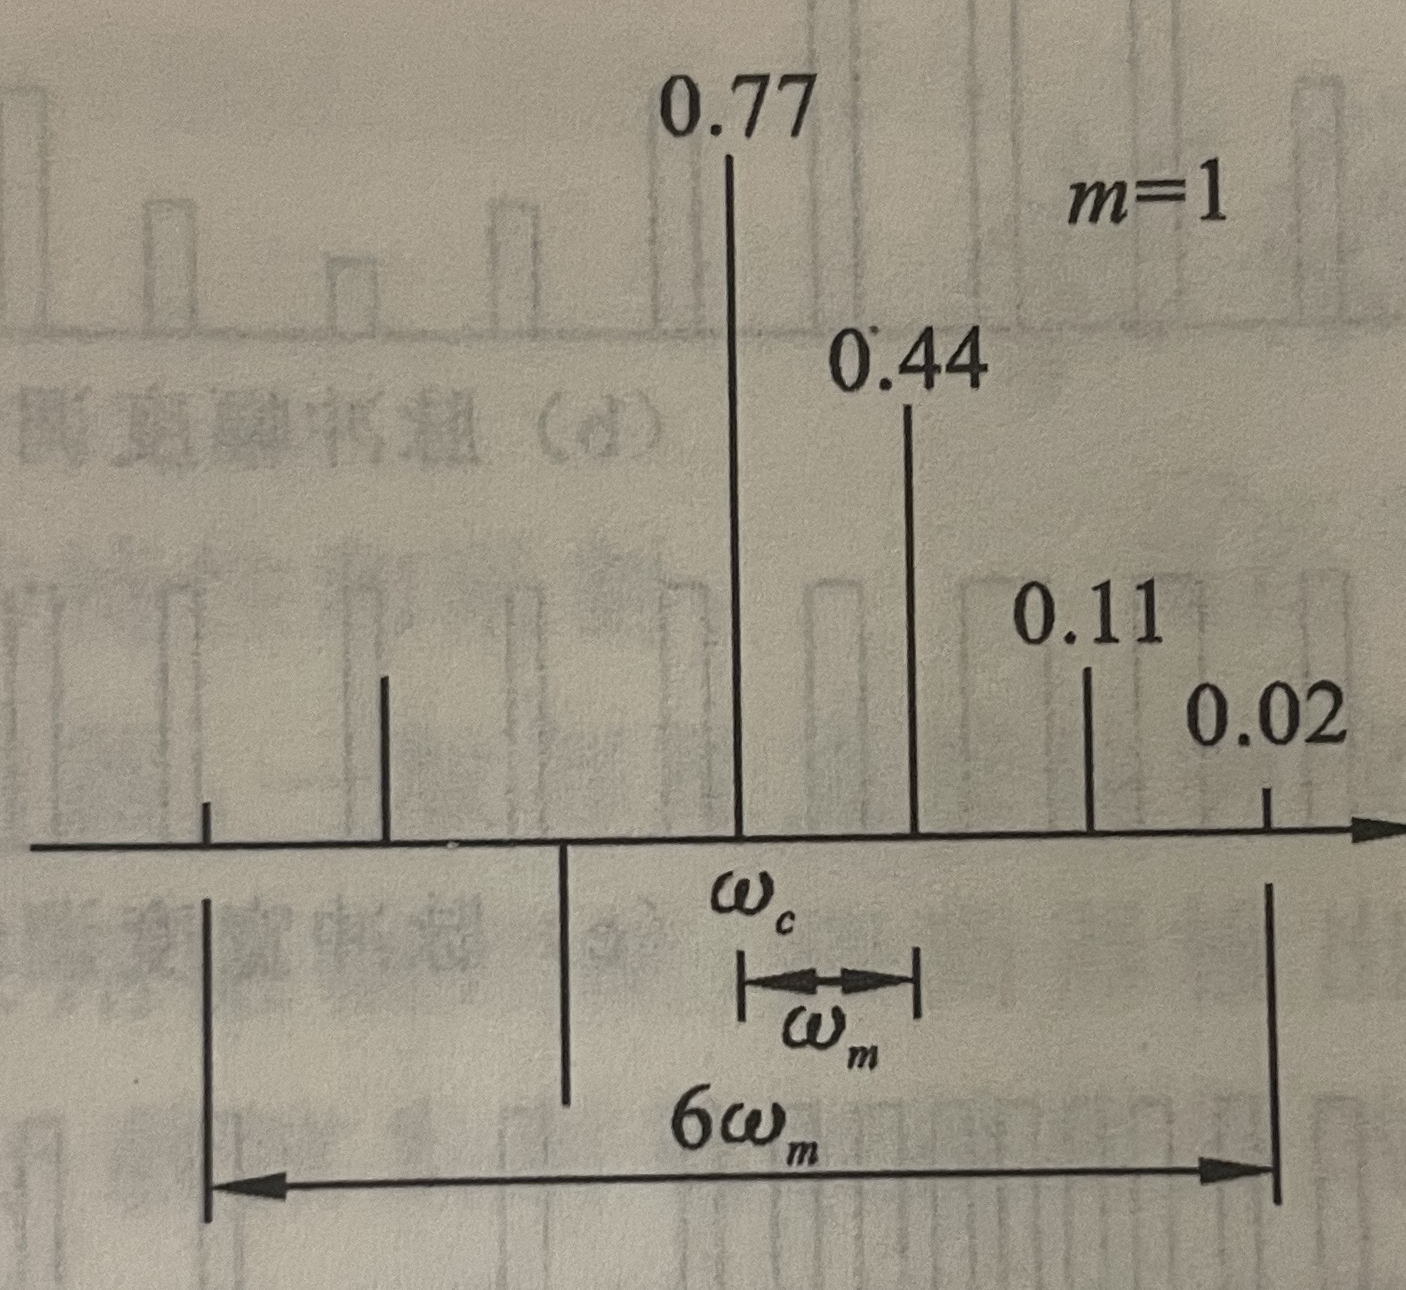
\includegraphics[width=0.3\textwidth]{EOMsidebandTheory.png}
    \caption{modulated laser beam frequency sepctrum}
    \label{fig:EOMsidebandTheory}
\end{figure}

 \subsubsection{EOM Tank Circuit Board: Model and Construction}



\section{Other Discussions}
\subsection{General Optical Lab Techniques and devices}
\begin{enumerate}
    \item discuss various optical devices on the optical table (reference QDevice content): wave plates, polarisers, etc -> briefly on how they work + how to use them in the lab 
    \begin{enumerate}
        \item wave plates, polarisers
        \item AR coating
        \item laser power meter: wavelength selection -> response curve
        \item lens cleaning
        \item DIY relevant tools in the lab. exmaples: strips of paper for ray tracing
        \item electronics stuff: soldering, PCB board inspection
        
    \end{enumerate}
\end{enumerate}


\section{Conclusion}
\begin{enumerate}
    \item what have I learn: about theory and experimental physics lab
    \item what have I done 
    \item possible follow up investigations / improvement on existing current
\end{enumerate}

\section{Acknowledgements}
thank the lab people! Jaren, Muyoung, Dzmitry, Nigel, Kowei

\section{Appendix}


\bibliographystyle{plain}
\bibliography{bibliography.bib}

\end{document}
